%Edit 0021 ZZZ to report number nnnn 
%Edit 3.1.2 YYMILE to milestone number m.m.m
%Edit Report on user frameworks for tokamak multiphysics YYTITLE to report title - Words Start with Caps
\documentclass[11pt,twoside,a4paper]{article}
%%======================================================================
%% PACKAGES:
%%
%\usepackage{times}               % Times+Helvetica+Courier fonts
\usepackage{helvet}              % helvetica + cmr
%\usepackage{frutiger}            % Frutiger \sffamily fonts.
\usepackage{fancyhdr}       % package for headers/footers
\usepackage{amsmath}
\usepackage{amssymb}
\usepackage{graphicx}            % Graphics.
%\usepackage{a4}                  % page layout to fit A4
%\usepackage{amssymb}              % 
%\usepackage{lastpage}            % get page no of last page
%\usepackage{ifthen}              % logical branching
\usepackage{hyperref}            %insert hyper-links
\usepackage{latexsym}
% uncomment the following to override auto page total
%\pptotal{20}
%%======================================================================

% ensure sans-serif font used throughout
\renewcommand{\familydefault}{\sfdefault}

\newcommand{\culhamissueno}{1.00}%<==edit
\newcommand{\culhamshorttitle}{CD/EXCALIBUR-FMS/0022}%<==edit
\newcommand{\Sec}[1]{Section~\ref{sec:#1}}
\newcommand{\Fig}[1]{Figure~\ref{fig:#1}}
\newcommand{\Eq}[1]{Equation~(\ref{eq:#1})}
\newcommand{\Eqs}[2]{Equations(\ref{eq:#1}) and~(\ref{eq:#2})}
\newcommand{\Figs}[2]{Figures~\ref{fig:#1}--~\ref{fig:#2}}
%Bold lc for script names, tt for computer code and file-names
%\F{NEPTUNE} always in caps
\newcommand{\F}[1]{\textsc{#1}}
\newcommand{\B}[1]{\textbf{#1}}
\newcommand{\T}[1]{{\tt #1}}
\newcommand{\V}[1]{\mathbf{#1}}
\newcommand{\I}[1]{\textit{#1}}
\newcommand{\nep}{\textsc{NEPTUNE}}
\newcommand{\exc}{\textsc{E}x\textsc{CALIBUR}}


%%======================================================================
%% REPORT COVER PAGE Information

\newcommand{\culhamtitle}{\LARGE Report on user layer design for
Uncertainty Quantification\\[1.0\baselineskip] M3.1.3 }%<==edit

%%qa box information -- change following as needed
%%only needed if uncomment approbox
\newcommand{\culhamboardname}{Martin O'Brien}%<==edit
\newcommand{\culhamcontactname}{Rob Akers}%<==edit
\newcommand{\culhamauthor}{Wayne Arter}%<==edit
\newcommand{\culhamauthora}{Lucian Anton}%<==edit
\newcommand{\culhamauthorb}{Debasmita Samaddar}%<==edit
\newcommand{\culhamauthorc}{\culhamcontactname}%<==edit
\newcommand{\culhamdate}{\today}%<=edit
\newcommand{\culhamdatea}{\today}%<=edit
\newcommand{\culhamdateb}{\today}%<=edit
%\newcommand{\culhamcontacttel}{Telephone: 01235 466498}
%\newcommand{\culhamcontactemail}{Email: rob.akers@ukaea.uk}

%
\setlength{\textheight}{290.0mm}
\setlength{\topmargin}{-20.0mm}
\setlength{\oddsidemargin}{-10.0mm}
\setlength{\evensidemargin}{\oddsidemargin}
\setlength{\parindent}{0mm}
\addtolength{\parskip}{0.5\baselineskip}
\setlength{\topsep}{0pt}
\setlength{\itemsep}{0pt}


\begin{document}

\begin{titlepage}

\includegraphics[width=2.5cm]{../corpics/cofaplus} \\[2.0\baselineskip]
{\LARGE {\textbf{\textsf{ExCALIBUR}}}}\\[2.0\baselineskip]
{\LARGE \culhamtitle } \\[2.0\baselineskip]
{\textbf{\textsf{Abstract}}}\\
The report describes work for \exc \ project \nep \
at Milestone M3.1.3.
This report describes techniques of uncertainty quantification~(UQ) that are expected
to prove important for \exc\ project \nep, arranged as they might appear in a
workflow to optimise device design.
First efficient ways of identifying the major sources of uncertainty
are identified, then second, techniques for working with this smaller number are described,
including the production of surrogates.
Third and lastly, UQ analysis is then continued with the
surrogates used to predict distributions of expected outcomes,
with emphasis on producing optimal device designs, which are robust
against say installation errors.\\
%Techniques described under the three headings are respectively\\
%%\begin{enumerate}
%1. Polynomial Chaos Expansion (PCE), Sparse regression (LASSO/Basis Pursuit), Multifidelity Monte-Carlo~(MFMC),
%Multilevel Monte-Carlo~(MLMC)  and Multi-Index Monte-Carlo~(MIMC)\\
%2. Adaptive, sparse quadrature sampling, Forward UQ and Sobol Analysis\\
%3. Surrogate models, Bayesian inference and Optimisation under uncertainty~(OUU)\\
%\end{enumerate}
Since \nep\ software
may be required for a range of applications including comparison with theory,
there is a discussion as to how UQ might best be integrated in the context of \nep, prior to completion
of UQ research work external to UKAEA.



\vfill
\hspace{-20mm}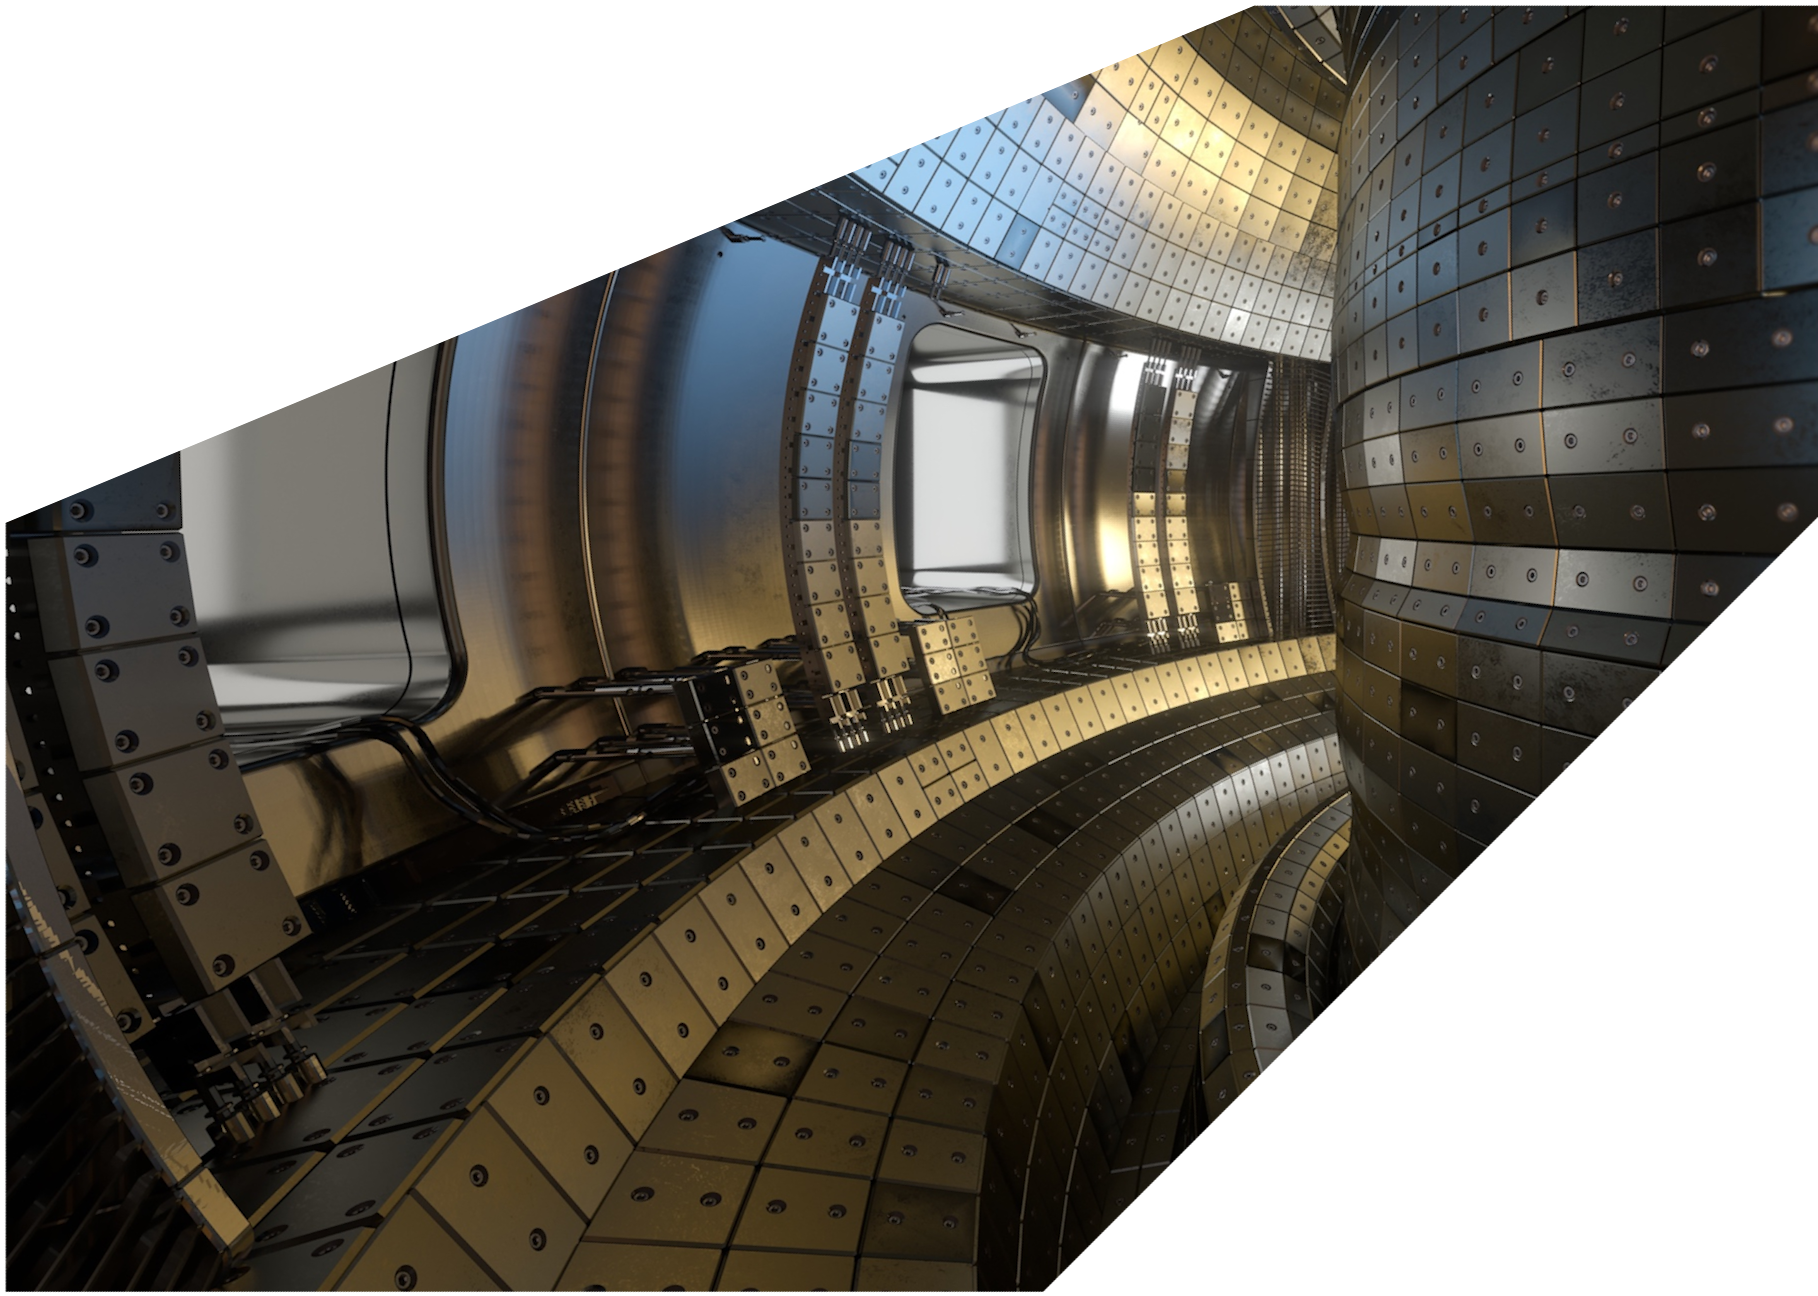
\includegraphics[width=18.0cm]{../corpics/tokintcrop}
\end{titlepage}

\clearpage
%\hspace{-30mm}\begin{table}[h]
\sffamily
\begin{center}
\textbf{\textsf{UKAEA REFERENCE AND APPROVAL SHEET}}
\begin{tabular}{||p{5.7cm}|p{4.7cm}|p{5.0cm}||}
\hline
\hline
& Client Reference: &  \\
\hline
& UKAEA Reference: & \culhamshorttitle \\
& & \\
\hline
& Issue: & \culhamissueno \\
\hline
& Date: & \culhamdateb \\
\hline
\multicolumn{3}{||l||}{} \\
\multicolumn{3}{||l||}{Project Name: ExCALIBUR Fusion Modelling System} \\
\multicolumn{3}{||l||}{} \\
\hline
\end{tabular}
\begin{tabular}{||p{3.3cm}|p{4.6cm}|p{3.5cm}|p{3.6cm}||}
\hline
& Name and Department & Signature & Date \\
\hline
Prepared By: & \culhamauthora & N/A & \culhamdate \\
& \culhamauthor & N/A & \culhamdate \\
%& \culhamauthorb  & N/A & \culhamdate \\
%& \culhamauthorc  & N/A & \culhamdate \\
& & & \\
& BD & & \\
\hline
Reviewed By: & \culhamcontactname & 
\includegraphics[width=3.0cm]{../corpics/blanksign}& \culhamdatea \\
& & & \\
& Advanced Computing Dept. Manager & & \\
\hline
%Approved By: & \culhamboardname  & \includegraphics[width=3.0cm]{../corpics/mobsign} & \culhamdateb \\
%& & & \\
%& MSSC & &\\
%\hline
\hline
\end{tabular}
\end{center}
\end{table}


\end{document}
